\section{Using Plugins}\index{plugins}

%% FIXME: here we need to include new python plugin section and updates

\subsection{An Introduction to Using Plugins}\label{label_introplugin}

QGIS has been designed with a plugin architecture.
This allows new features/functions to be added to the application.
Many of the features in QGIS are actually implemented as plugins.

There are two types of plugins in QGIS: core and user-contributed.
\index{plugins!types} A core plugin is maintained by the QGIS development team and is part of every QGIS distribution.
A user-contributed plugin is an external plugin that is maintained by the individual author.
The QGIS SVN website (\url{http://svn.qgis.org}) serves some user contributed plugins.

\subsubsection{Finding and Installing a Plugin}
When you install QGIS, all of the core plugins are included (see chapter \ref{sec:core_plugins}). \index{plugins!installing}
% Additional user-contributed
% plugins may be available on the QGIS Community site. To see what
% user-contributed plugins are available, see the plugins page on the Community
% site (\url{http://community.qgis.org/plugins}).\index{plugins!user
% contributed}

Typically user-contributed plugins are distributed in source form and require compiling.
For instructions on building and installing a user-contributed plugin, see the documentation included with the plugin.

\subsubsection{Managing Plugins}\label{sec:managing_plugins}
\index{plugins!managing} Managing plugins consists of loading or unloading them from QGIS.
Loaded plugins are "remembered" when you exit the application and restored the next time you run QGIS.

To manage plugins, open \mainmenuopt{Plugins} > \dropmenuopttwo{mActionShowPluginManager}{Plugin Manager...}
\index{plugins!manager}The Plugin Manager displays all the available plugins and their status (loaded or unloaded).
Figure \ref{fig:pluginmanager} shows the Plugin Manager dialog.

%\begin{figure}[ht]
%   \begin{center}
%   \caption{Plugin Manager}\label{fig:pluginmanager}\smallskip
%   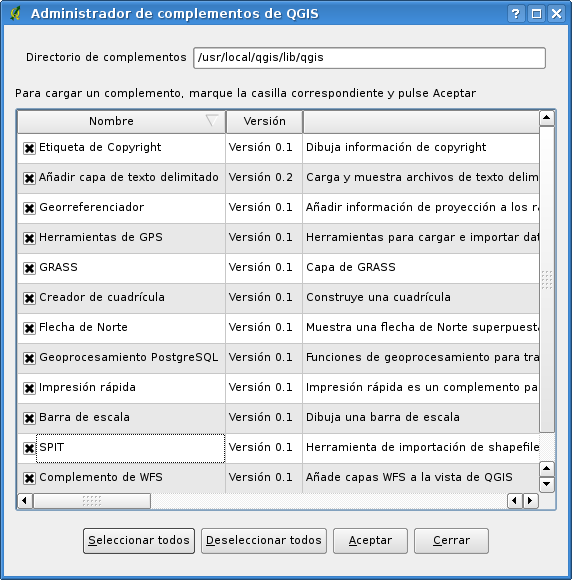
\includegraphics[clip=true, width=14cm]{pluginmanager2}
%\end{center}  
%\end{figure}

Typically all QGIS plugins are installed in the same location.
This location is shown in the Plugin Directory text field.
You can tell QGIS to load plugins from another location by specifying a different directory.

\begin{Tip}\caption{\textsc{Crashing Plugins}}\index{crashes}
\qgistip{If you find that QGIS crashes on startup, a plugin may be at fault.
You can stop all plugins from loading by editing your stored settings file (see \ref{subsec:gui_options} for location).
Locate the plugins settings and change all the plugin values to false to prevent them from loading.
\nix {For example, to prevent the Delimited text plugin from loading, the entry in \$HOME/.config/QuantumGIS/qgis.conf on Linux 
should look like this:\ttfamily{Add Delimited Text Layer=false}.}
\normalfont 
Do this for each plugin in the [Plugins] section.
You can then start QGIS and add the plugins one at a time from the Plugin Manger to determine which is causing the problem.
}
\end{Tip} 

\subsubsection{Data Providers}\index{data providers}

Data Providers are "special" plugins that provides access to a data store.
By default, QGIS supports PostGIS layers and disk-based data stores supported by the GDAL/OGR library (Appendix \ref{appdx_ogr}).
A Data Provider plugin extends the ability of QGIS to use other data sources.

Data Provider plugins are registered automatically by QGIS at startup.
They are not managed by the Plugin Manager but are used behind the scenes when a corresponding data type is added as a layer in QGIS.

\subsubsection{Core Plugins}\label{sec:core_plugins}\index{plugins!core}

QGIS currently contains 12 core plugins that can be loaded using the Plugin Manager.
Table \ref{tab:core_plugins} lists each of the core plugins along with a description of their purpose and the toolbar-icon.
Note the GRASS plugin is not included below because it installs its own toolbar (see section \ref{sec:grass} for a discussion of available features in the GRASS plugin).

% minipage is needed to appear the footnote under the table
% SH
\begin{minipage}{\textwidth}
\begin{table}[H]
\centering
\caption{QGIS Core Plugins}\label{tab:core_plugins}\medskip
\small
 \begin{tabular}{|l|l|p{4in}|}
\hline \textbf{Icon} & \textbf{Plugin} & \textbf{Description} \\
\hline 
% WHICH ICON TO CHOOSE HERE?

\includegraphics[width=0.7cm]{plugins_delimited_text_images/delimited_text}
 & Delimited Text \index{plugins!delimited text}& Load a delimited text file containing x,y coordinates as a point layer \\
\hline 

\includegraphics[width=0.7cm]{plugins_decorations_images/copyright_label}
 & Copyright Label \index{plugins!copyright}& Display a copyright label on the map canvas\\
\hline 

\includegraphics[width=0.7cm]{plugins_gps_images/gps_importer}
 & GPS Tools \index{plugins!gps}& Load and display GPS data \\
\hline
% WHICH ICON TO CHOOSE HERE?

\includegraphics[width=0.7cm]{plugins_grass_module_images/grasslogo}
 & GRASS Toolbox \index{plugins!grass}& The most important GRASS functionality \\
\hline
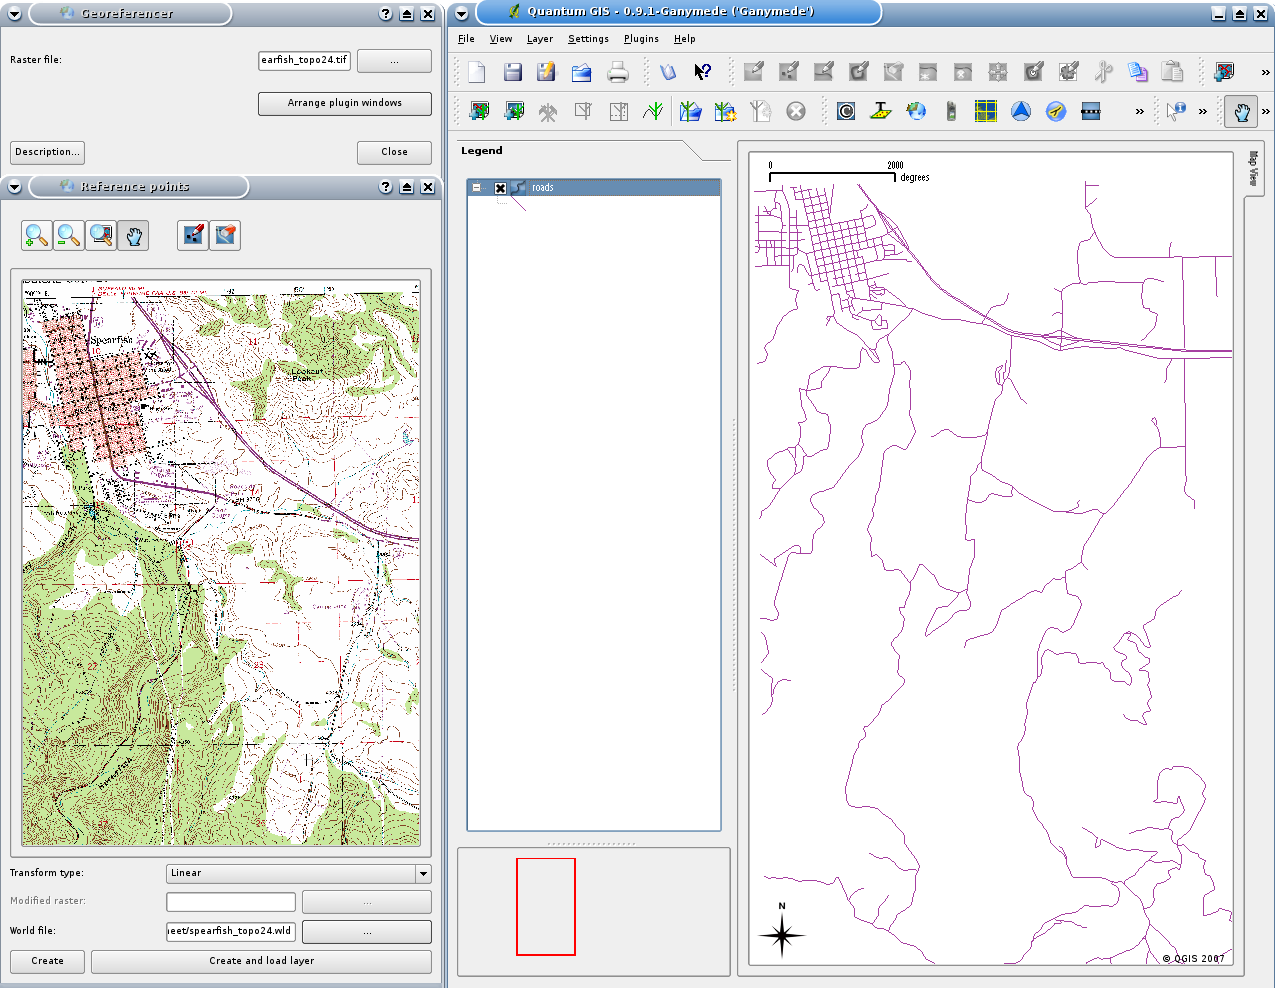
\includegraphics[width=0.7cm]{plugins_georeferencer_images/georeferencer}
 & Georeferencer \index{plugin!georeferencer} & Georeferencing rasterlayers \\
\hline

\includegraphics[width=0.7cm]{plugins_graticule_creator_images/grid_maker}
 & Graticule Creator \index{plugins!graticule}& Create a latitude/longitude grid and save as a shapefile\\
\hline
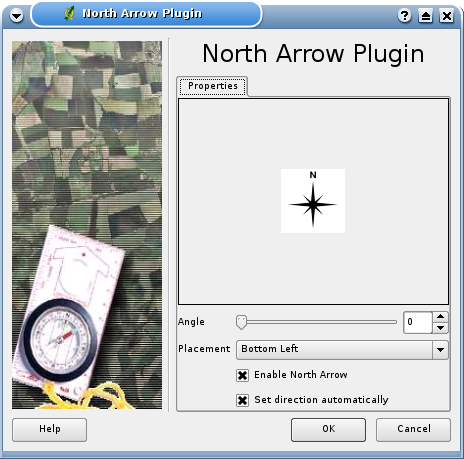
\includegraphics[width=0.7cm]{plugins_decorations_images/north_arrow}
& North Arrow \index{plugins!north arrow}& Add a north arrow to the map canvas\\
\hline

\includegraphics[width=0.7cm]{plugins_geoprocessing_images/icon_buffer}
 & PostgreSQL Geoprocessing \index{plugins!geoprocessing}& Buffer a PostGIS layer \\
\hline

\includegraphics[width=0.7cm]{plugins_quick_print_images/quick_print}
 & Quick Print \index{plugins!quickprint}& Quickly print a map \\
\hline
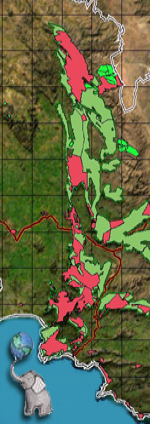
\includegraphics[width=0.7cm]{plugins_spit_images/spit}
 & SPIT \index{plugins!spit}& Shapefile to PostGIS Import Tool - import shapefiles into PostgreSQL\\
\hline

\includegraphics[width=0.7cm]{plugins_decorations_images/scale_bar}
 & Scalebar \index{plugins!scalebar}& Add a scalebar to the map canvas\\
\hline 

\includegraphics[width=0.7cm]{plugins_add_wfs_layer_images/mIconAddWfsLayer}
 & WFS & Load and display WFS layer \\
\hline
\end{tabular}
\end{table}
\end{minipage}

\normalsize


\begin{Tip}\caption{\textsc{Plugins Settings Saved to Project}}\index{plugins
settings}
\qgistip{When you save a .qgs project, any changes you have made to NorthArrow, ScaleBar and Copyright plugins will be saved in the project and restored next time you load the project.
}
\end{Tip}

%
% External Plugins
%
\subsubsection{External Plugins}\label{sec:external_plugins}\index{plugins!external}

QGIS also comes with some externally developed plugins.
They are not shipped with the default distribution.
However, they can be compiled and used within QGIS.

Currently the external plugins are only available directly from SVN.
To check out all available external plugins do the following:
\begin{verbatim}
svn co https://svn.osgeo.org/qgis/trunk/external_plugins external_qgis_plugins
\end{verbatim}

This will create a folder \texttt{external\_qgis\_plugins} in your current folder.
Each subdirectory has its own compile and install instructions.
Read them carefully in order to build the plugin.

%
% Plugin template
%
\subsubsection{Plugin templates}\label{sec:plugin_template}\index{plugins!template}

If you like to develop your own QGIS-plugin the main sources include a nice script which guides you through the process of creating your own template-directory-structure within the QGIS-source-tree.
The script lives in \texttt{QGIS/src/plugins/plugin\_builder.pl}.

The only thing to do is coding your functions into the plugin (and of course contribute your plugin to the QGIS-development-team).

Beside that the QGIS-wiki (\url{http://wiki.qgis.org}) and the QGIS-blog (\url{http://blog.qgis.org}) provide useful articles about writing your own plugin as well.
Check the websites for details!
